\documentclass[10pt,xcolor={dvipsnames}]{beamer}
\usetheme[
%%% option passed to the outer theme
%    progressstyle=fixedCircCnt,   % fixedCircCnt, movingCircCnt (moving is deault)
  ]{Feather}
  
% If you want to change the colors of the various elements in the theme, edit and uncomment the following lines

% Change the bar colors:
\setbeamercolor{Feather}{fg=NavyBlue!20,bg=NavyBlue}

% Change the color of the structural elements:
\setbeamercolor{structure}{fg=NavyBlue}

% Change the frame title text color:
\setbeamercolor{frametitle}{fg=black!5}

% Change the normal text colors:
\setbeamercolor{normal text}{fg=black!75,bg=gray!5}

%% Change the block title colors
\setbeamercolor{block title}{use=Feather,bg=Feather.fg, fg=black!90} 


% Change the logo in the upper right circle:
%\renewcommand{\logofile}{example-grid-100x100pt} 
%% This is an image that comes with the LaTeX installation
% Adjust scale of the logo w.r.t. the circle; default is 0.875
% \renewcommand{\logoscale}{0.55}

% Change the background image on the title and final page.
% It stretches to fill the entire frame!
% \renewcommand{\backgroundfile}{example-grid-100x100pt}

%-------------------------------------------------------
% INCLUDE PACKAGES
%-------------------------------------------------------

\usepackage[utf8]{inputenc}
\usepackage[english]{babel}
\usepackage[T1]{fontenc}
% \usepackage{helvet}

%% Load different font packages to use different fonts
%% e.g. using Linux Libertine, Linux Biolinum and Inconsolata
% \usepackage{libertine}
% \usepackage{zi4}

%% e.g. using Venturis ADF Serif and Sans
% \usepackage{venturis}

%-------------------------------------------------------
% DEFFINING AND REDEFINING COMMANDS
%-------------------------------------------------------

% colored hyperlinks
\newcommand{\chref}[2]{
  \href{#1}{{\usebeamercolor[bg]{Feather}#2}}
}

%-------------------------------------------------------
% INFORMATION IN THE TITLE PAGE
%-------------------------------------------------------

\title[Fund Computación] % [] is optional - is placed on the bottom of the sidebar on every slide
{ % is placed on the title page
      \Large{\textbf{Fundamentación en computación}}
}

\subtitle[Taller 1]
{
      \textbf{Una herramienta científica inevitable}
}

\author[Julián Calle]
{      Julián Calle \\
      {\ttfamily julian.callem@udea.edu.co}\\[1em]
      Taller 1
}

\institute[UdeA]
{%
\begin{columns}
\begin{column}{3cm}

\includegraphics[scale=0.045]{Feathergraphics/2-2} 
\end{column}
\begin{column}{6cm} 
Instituto de física\\
Facultad de ciencias exactas y naturales \\
Universidad de Antioquia
\end{column} \end{columns}
}

\date{\today}

%-------------------------------------------------------
% THE BODY OF THE PRESENTATION
%-------------------------------------------------------

\begin{document}

%-------------------------------------------------------
% THE TITLEPAGE
%-------------------------------------------------------

{\1
\begin{frame}[plain,noframenumbering]
  \titlepage
\end{frame}}


%\begin{frame}{Content}{}
%\tableofcontents
%\end{frame}

\begin{frame}{Repositorio del curso}
\begin{center}

\includegraphics[scale=0.3]{Figures/BobSponge} \pause
\url{https://jacallem94.github.io/Fund-Computacion/}
\end{center}
\end{frame}

\begin{frame}
\begin{center}
\Huge{\textcolor{blue}{Importancia de la computación en la ciencia}}
\end{center}
\end{frame}

\begin{frame}{Computación en física}
\begin{center}
\only<2->{La experimentación es indispensable en física.}
\only<3>{
\includegraphics[scale=0.2]{Figures/Homero}}
\only<4->{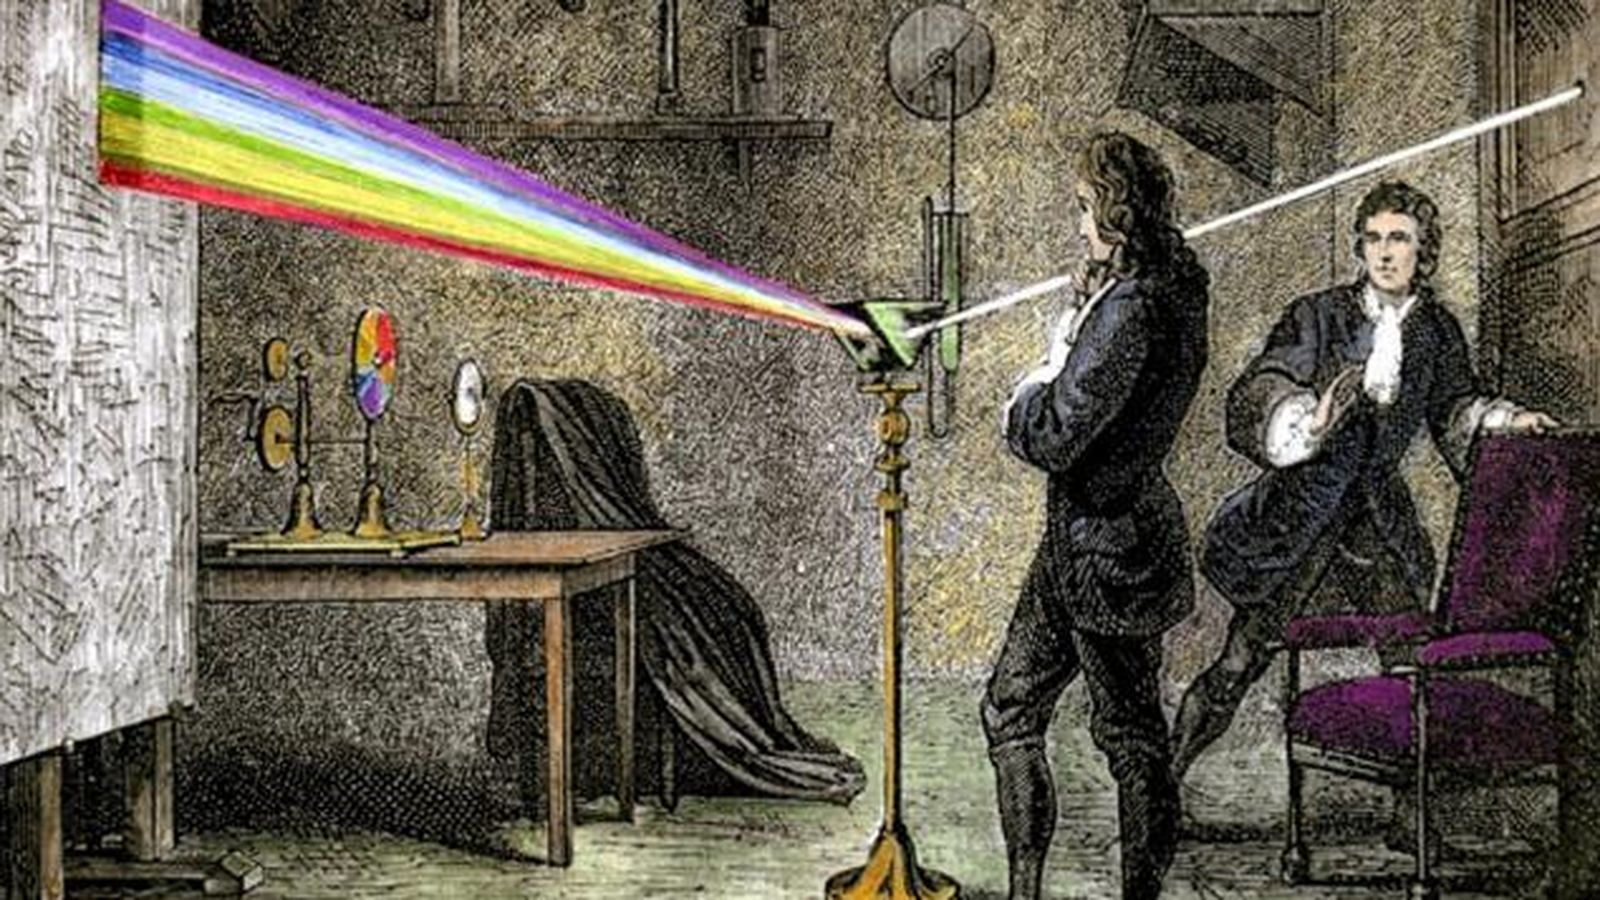
\includegraphics[scale=0.15]{Figures/Experimento}}
\only<5>{\url{https://phet.colorado.edu/sims/html/pendulum-lab/latest/pendulum-lab_es.html}}
\only<6>{\url{https://phet.colorado.edu/sims/html/gases-intro/latest/gases-intro_es.html}}
\only<7>{\url{https://phet.colorado.edu/sims/html/wave-interference/latest/wave-interference_es.html}}
\end{center}
\end{frame}

\begin{frame}{Computación en física}
\begin{center}
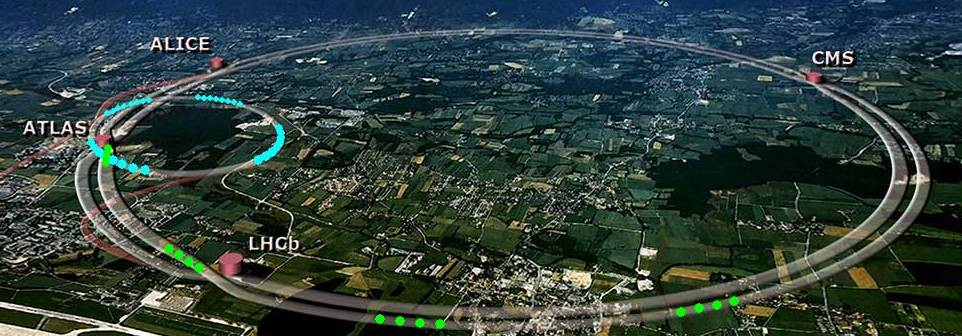
\includegraphics[scale=0.3]{Figures/LHC}
LHC
\end{center}
\end{frame}

\begin{frame}{Computación en física}
\begin{center}
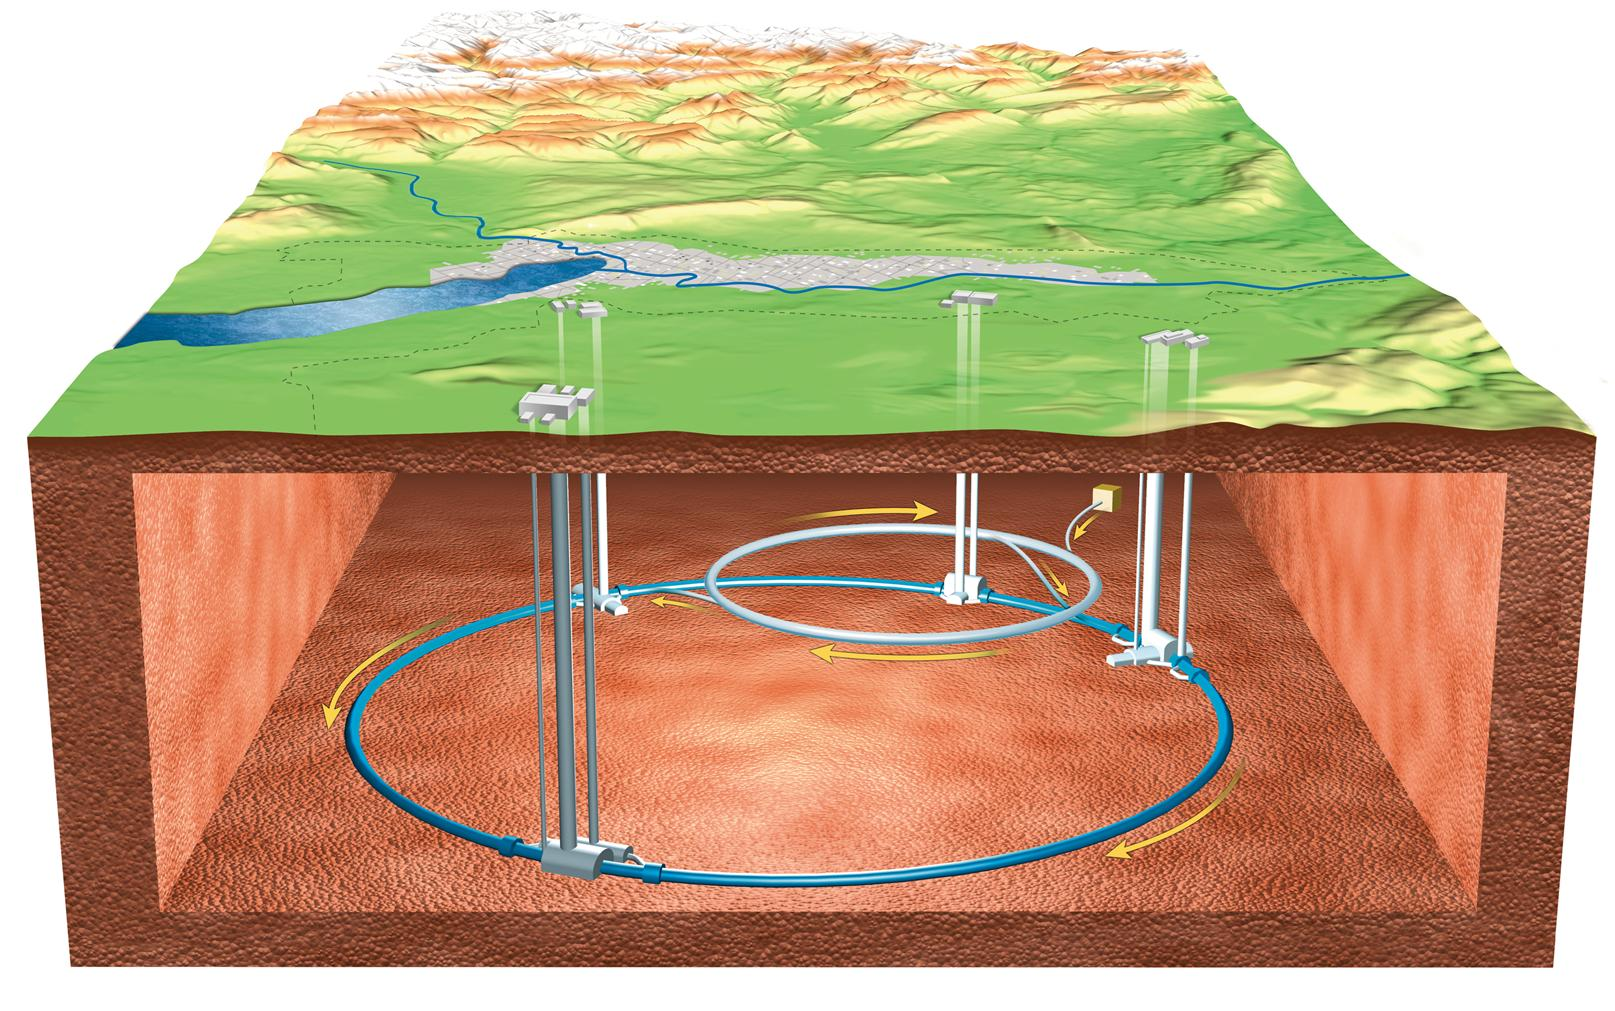
\includegraphics[scale=0.38]{Figures/bajotierra}
\end{center}
\end{frame}


\begin{frame}{Computación en física}
\begin{center}
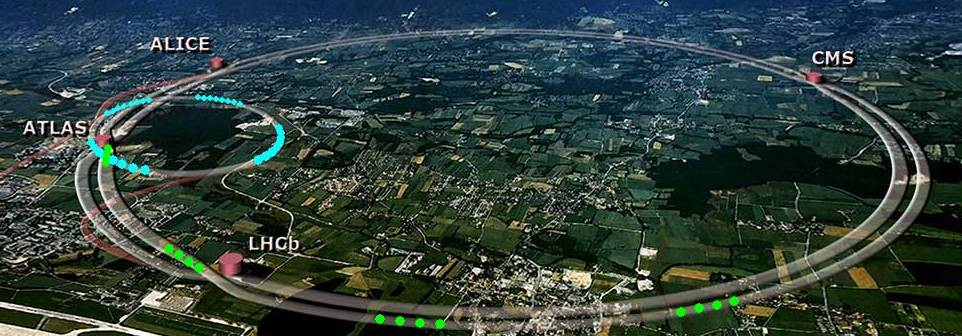
\includegraphics[scale=0.3]{Figures/LHC}
LHC
\end{center}
\end{frame}

\begin{frame}{Computación en física}
\begin{center}
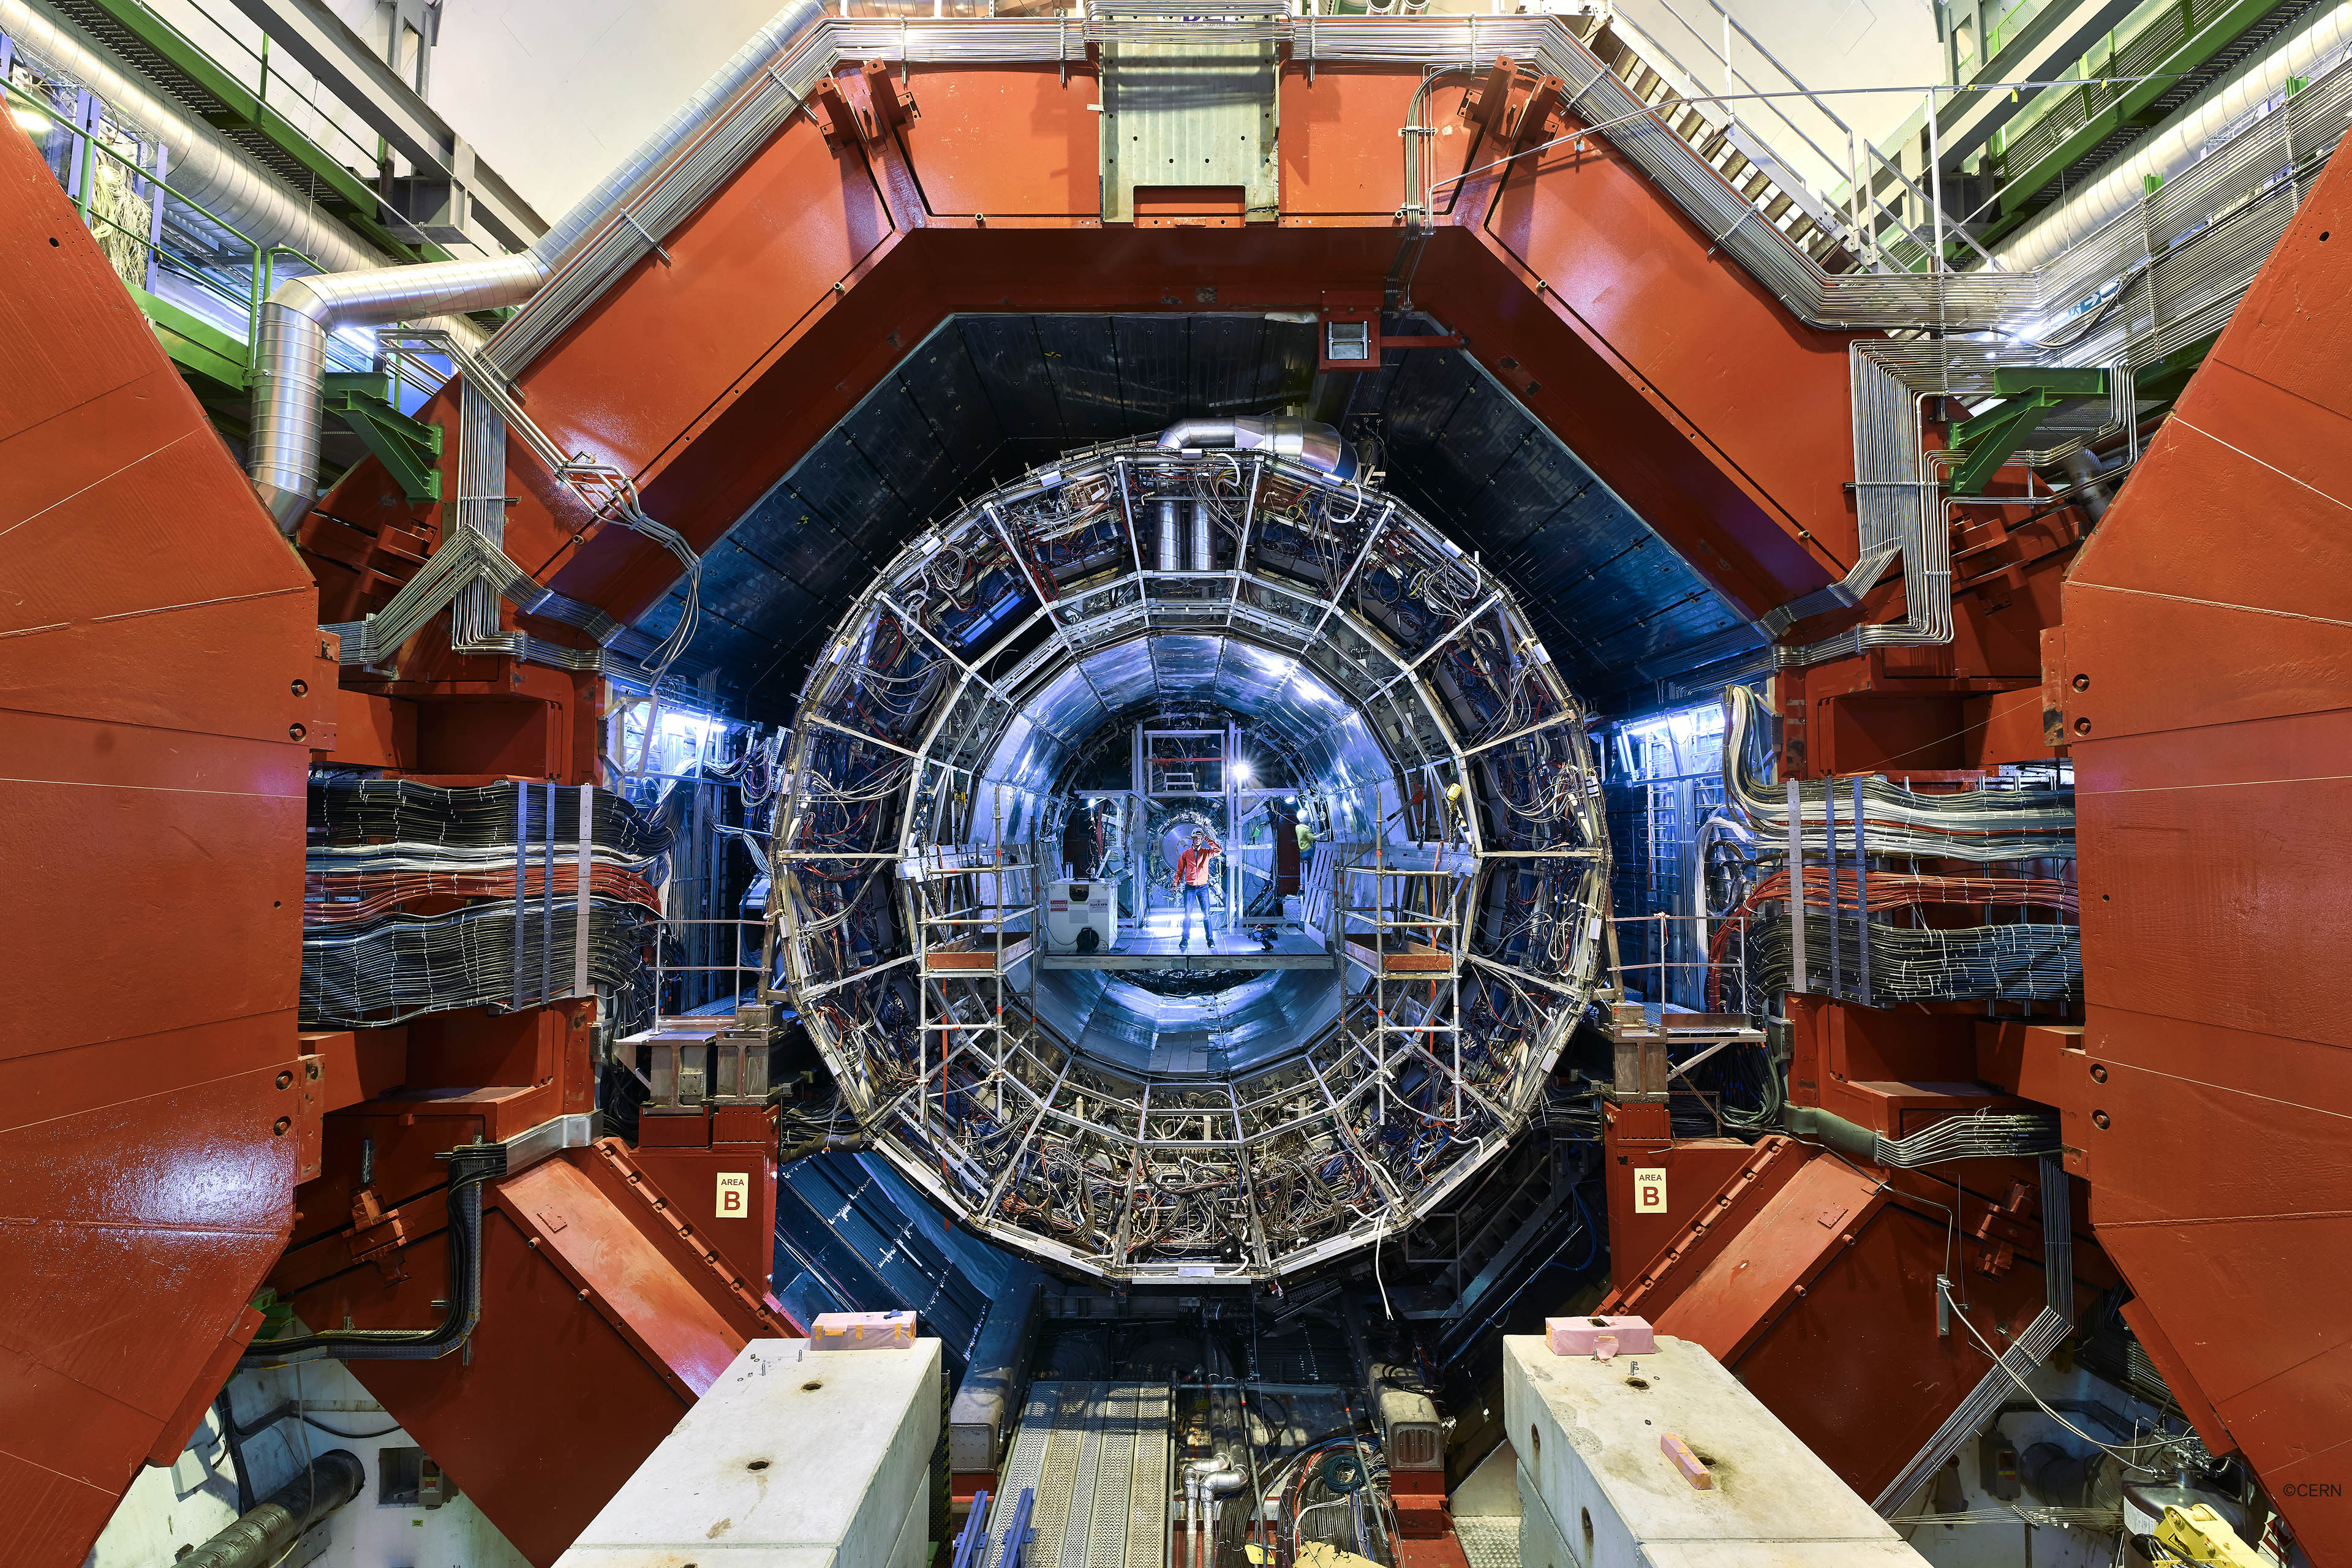
\includegraphics[scale=0.13]{Figures/ALICE}
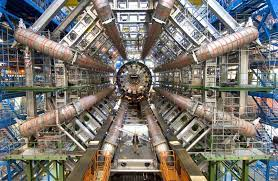
\includegraphics[scale=0.43]{Figures/Atlas} \\
ALICE \hspace{4cm} ATLAS \\ \vspace{0.5cm}
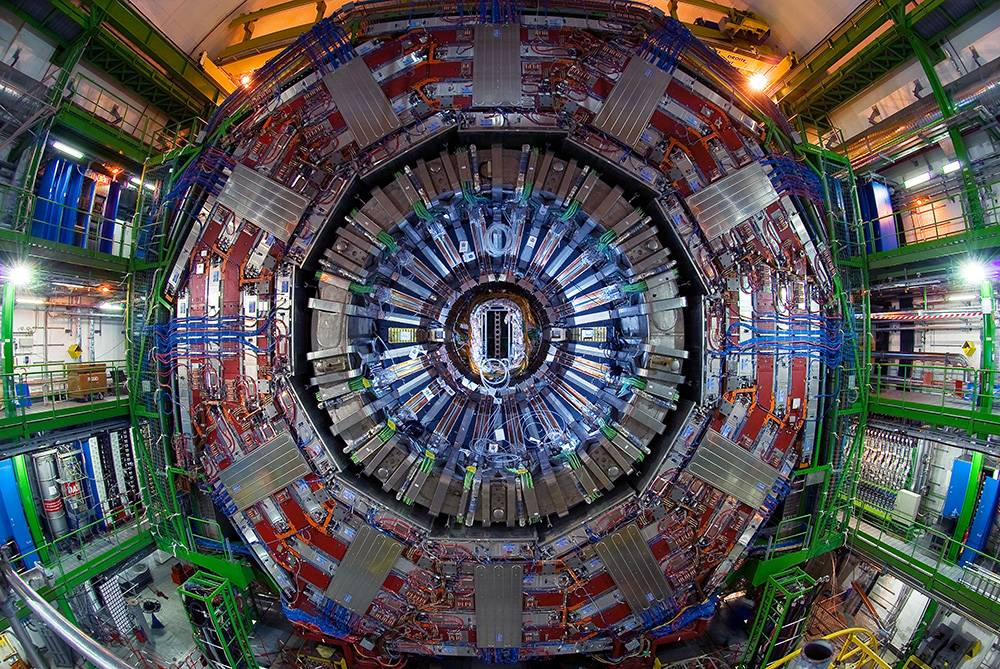
\includegraphics[scale=0.13]{Figures/CMS}
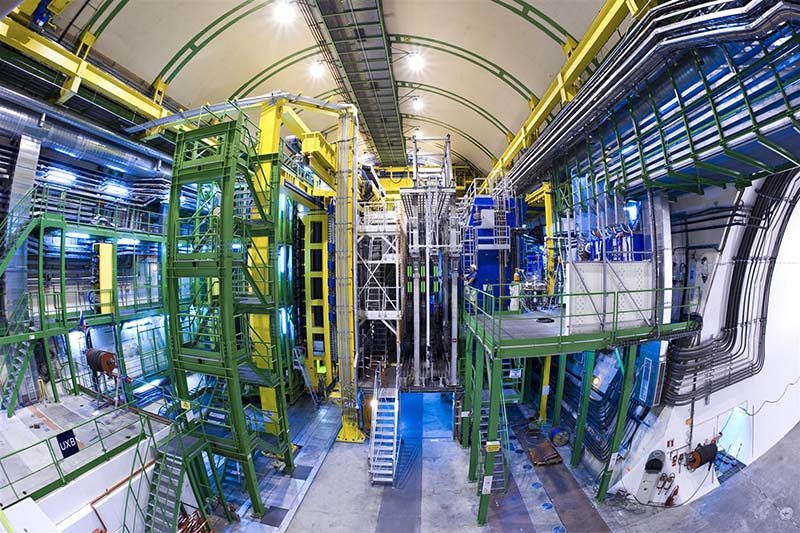
\includegraphics[scale=0.43]{Figures/LHCb} \\
CMS \hspace{4cm} LHCb
\end{center}
\end{frame}

\begin{frame}{Computación en física}
\begin{center}
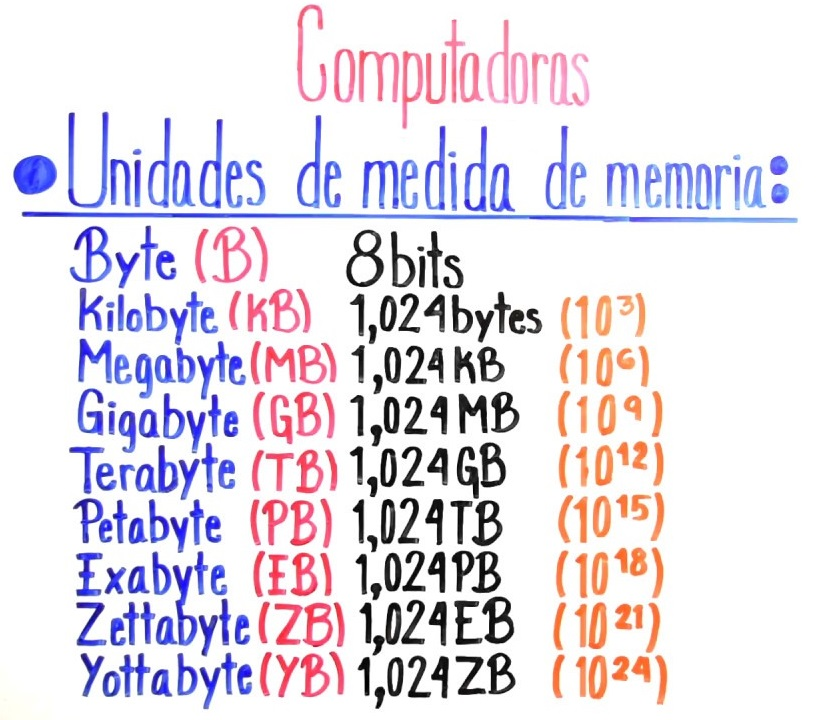
\includegraphics[scale=0.38]{Figures/unidades-de-medida-en-computacion}
\end{center}
\end{frame}

\begin{frame}{Computación en física}
\begin{center}
\Large{\textcolor{blue}{Bosón de Higgs}} \\
\only<2>{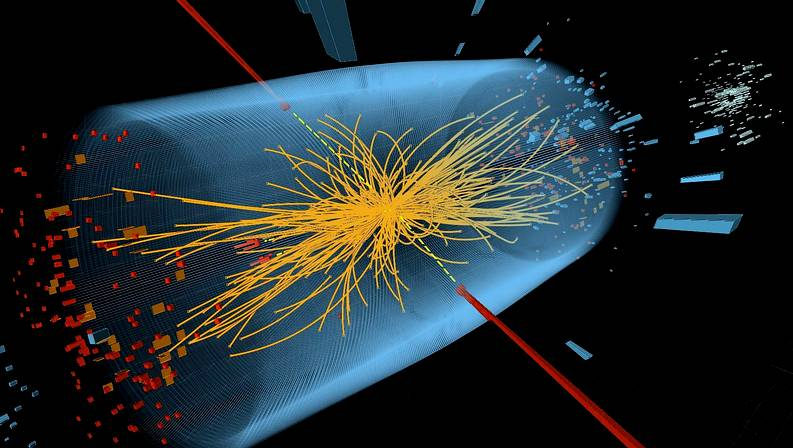
\includegraphics[scale=0.4]{Figures/HiggsCol}}
\only<3>{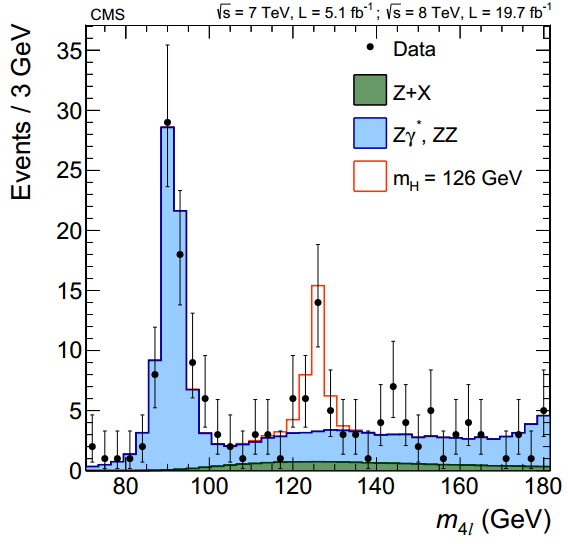
\includegraphics[scale=0.4]{Figures/Higgs}}
\end{center}
\end{frame}

\begin{frame}{Computación en astronomía}
\begin{center}
\only<2>{\Huge{\textcolor{red}{¿Cómo experimentar en astronomía?}}}
\only<3->{La astronomía es una maquina del tiempo.}
\only<4>{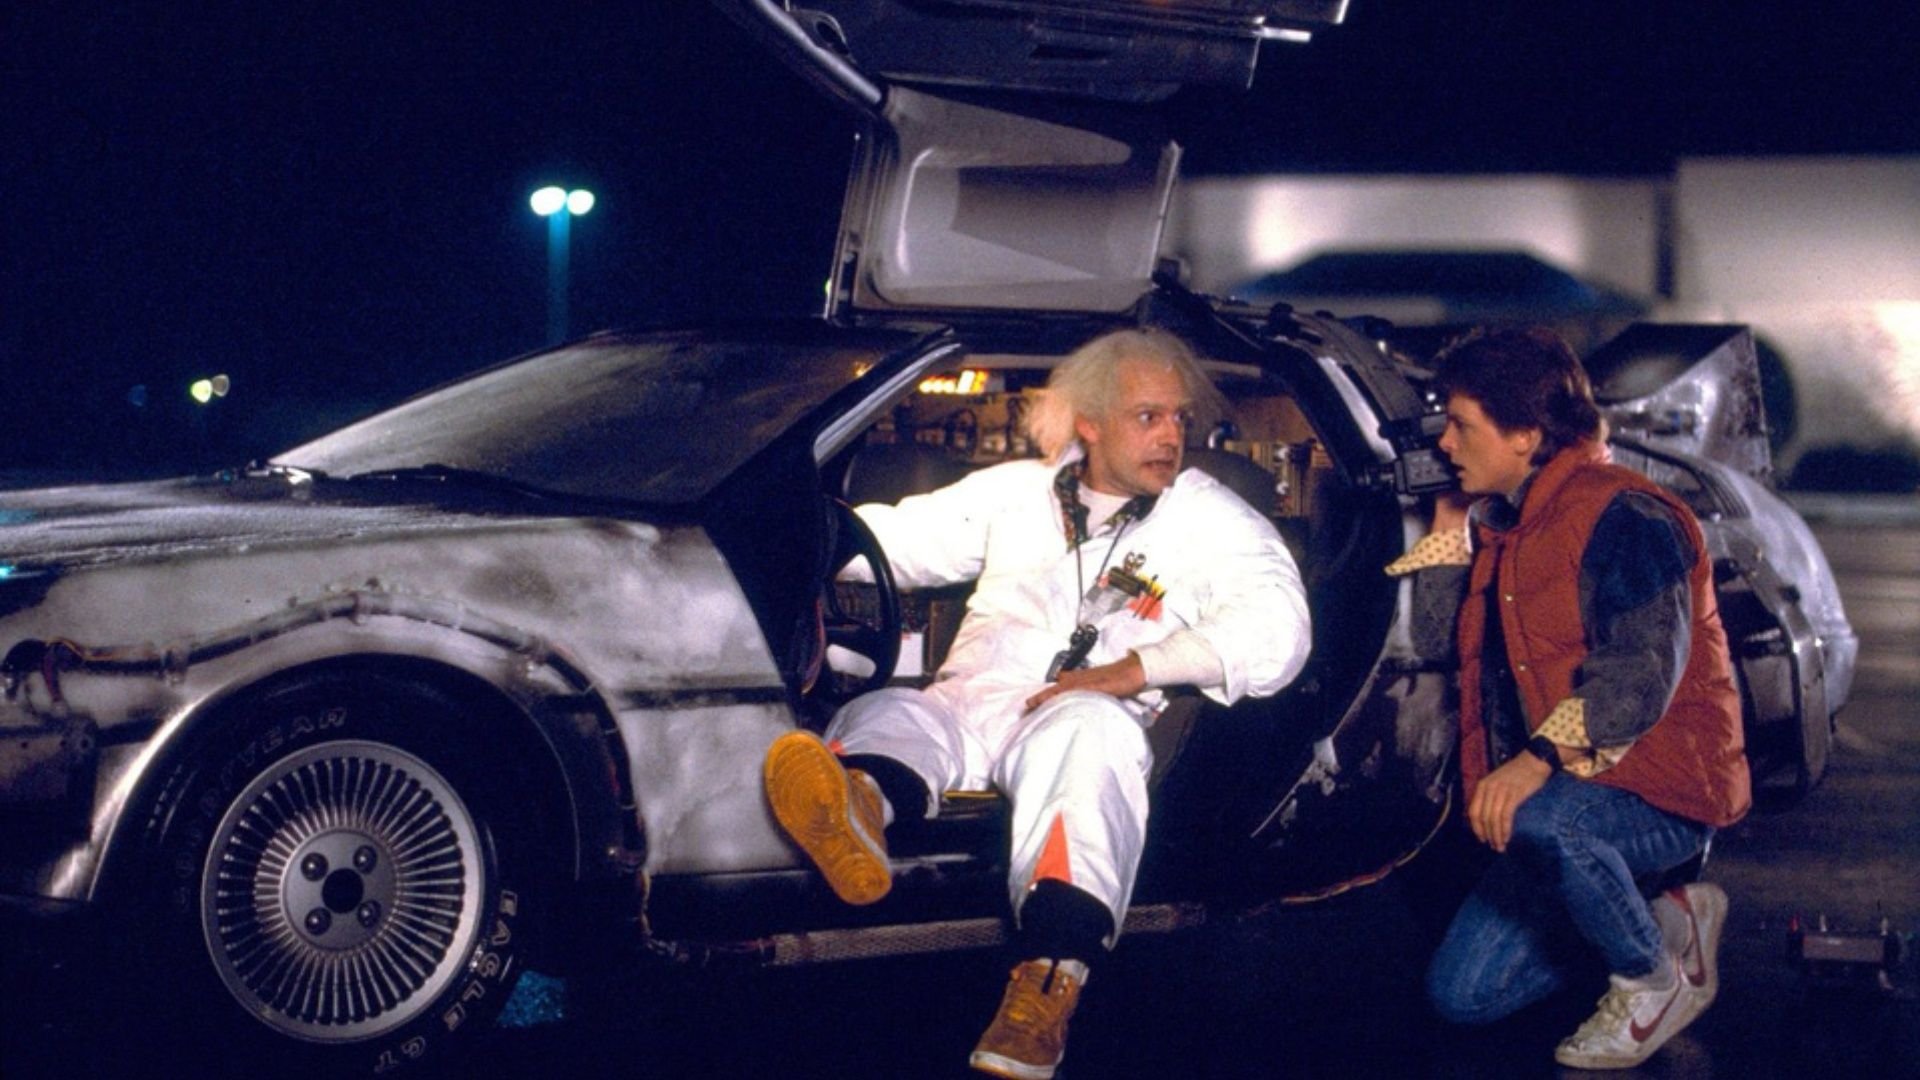
\includegraphics[scale=0.2]{Figures/delorean}}
\only<5>{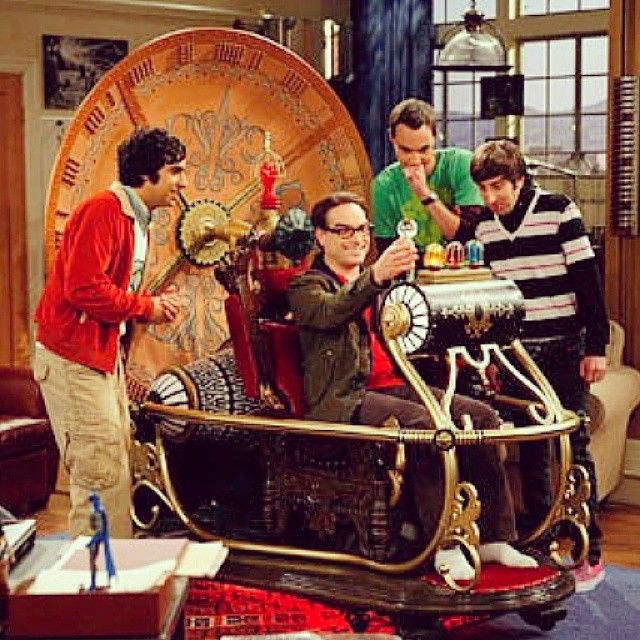
\includegraphics[scale=0.28]{Figures/Bigbang}}
\end{center}
\end{frame}

\begin{frame}{Computación en astronomía}
\begin{center}
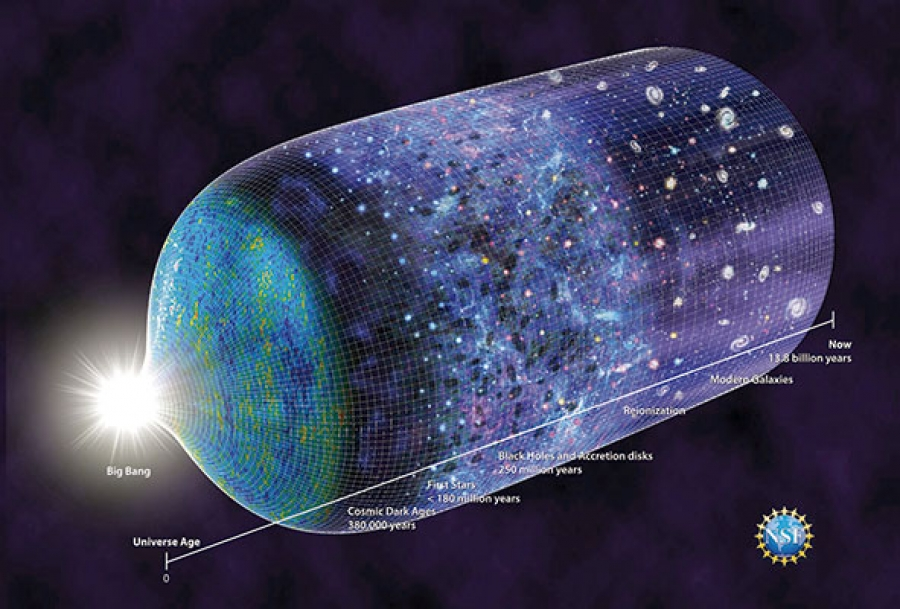
\includegraphics[scale=0.3]{Figures/Cosmologia}
\end{center}
\end{frame}


\begin{frame}{Computación en astronomía}
\begin{center}
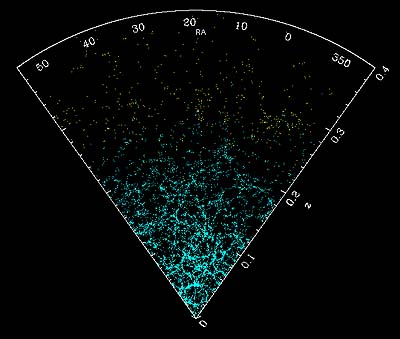
\includegraphics[scale=0.5]{Figures/Cosmo}
\end{center}
\end{frame}


\begin{frame}{Computación en astronomía}
\begin{center}
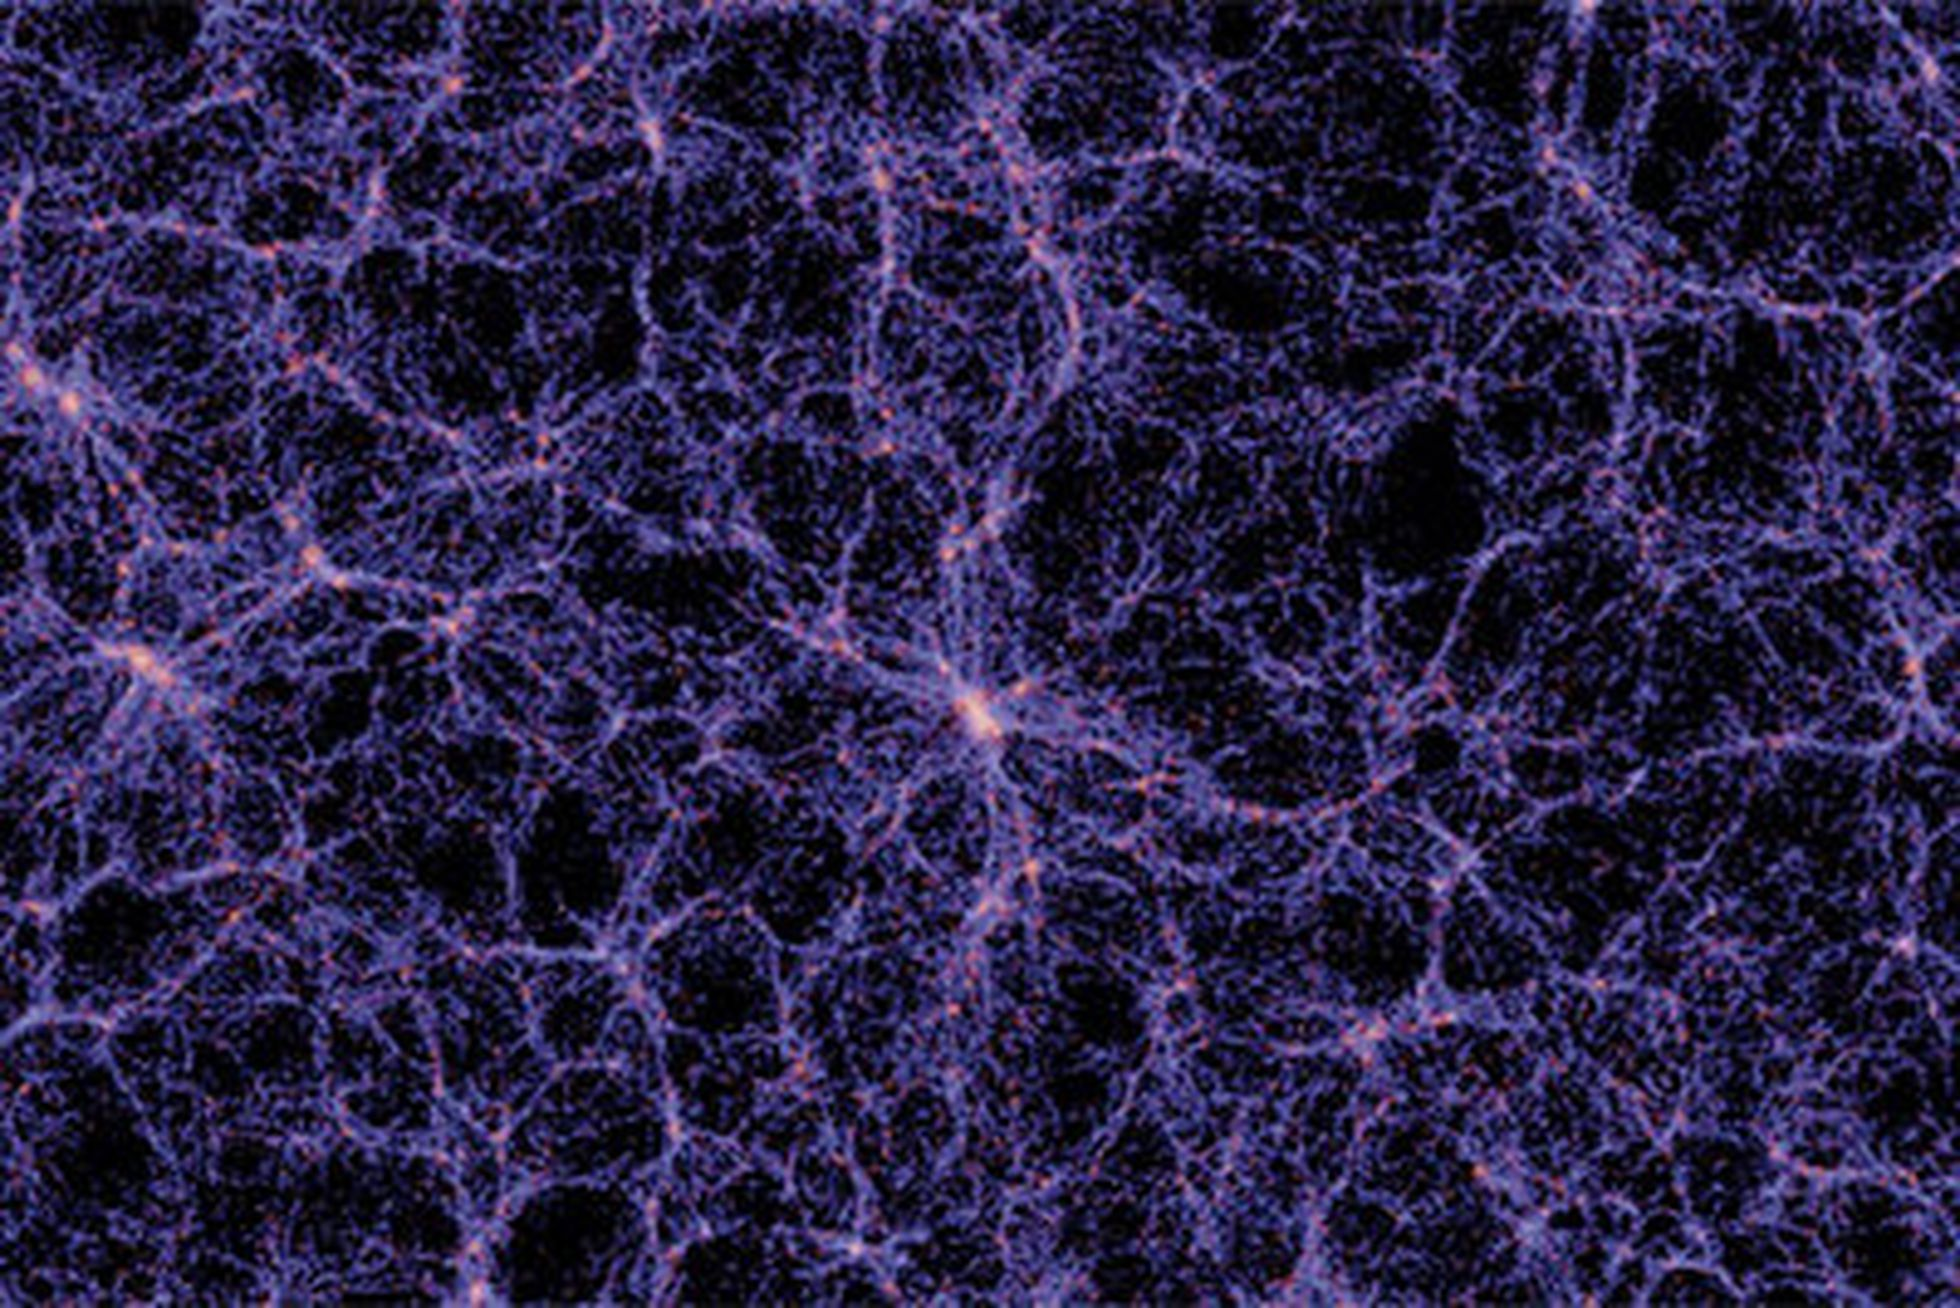
\includegraphics[scale=0.13]{Figures/SimMilenio} \pause
\url{https://youtu.be/vHApMrssVJM}
\end{center}
\end{frame}


\begin{frame}{Computación en astronomía}
\begin{center}
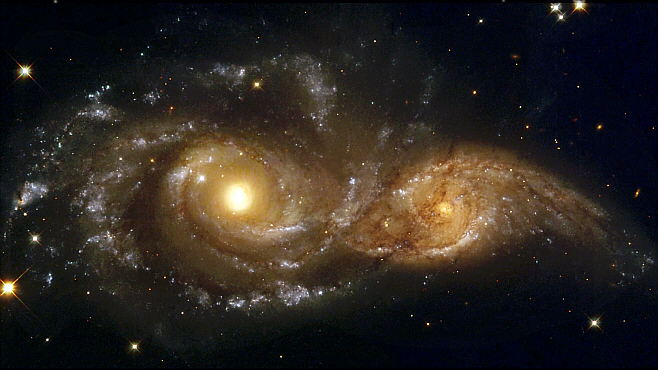
\includegraphics[scale=0.5]{Figures/colisgal} \pause
\url{https://youtu.be/XFYqEMN9ooI}
\end{center}
\end{frame}


\begin{frame}{Computación en astronomía}
\begin{center}
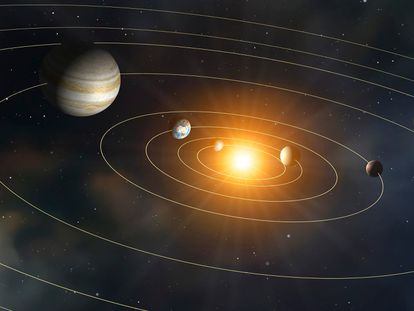
\includegraphics[scale=0.6]{Figures/sistemasolar}
\only<2>{\url{https://stellarium-web.org/}}
\only<3>{\url{https://www.solarsystemscope.com/ }}
\only<4>{\url{https://stellarium.org/es/}}
\end{center}
\end{frame}

\begin{frame}{Wolfram}
\begin{center}

\includegraphics[scale=0.3]{Figures/Wolfram} \pause \\ 
\url{https://www.wolframalpha.com/}
\end{center}
\end{frame}

\begin{frame}{Cuestionario}
\begin{center}

\includegraphics[scale=0.18]{Figures/BobS} \pause
\url{https://forms.gle/j2fkoXVJceHr69Pg8}
\end{center}
\end{frame}


{\1
\begin{frame}[plain,noframenumbering]
  \finalpage{
\includegraphics[scale=0.5]{Figures/Meme}}
\end{frame}}

\end{document}